%!TEX root = ../MasterThesis.tex

\section{Scenario Description}
\label{sec:scenario_description}

E-commerce as a term relates to the trading of products or services utilizing a computer network such as the Internet. It is usually categorized into the following four different subfields \citep{sen2015study}:\@

\begin{enumerate}
  \item \textbf{Business-To-Business (B2B)}: refers to electronic trading between companies with the objective to improve their supply chain processes
  \item \textbf{Business-To-Consumer (B2C)}: refers to electronic trading between a company and it's consumers (most publicly known example is Amazon)
  \item \textbf{Consumer-To-Consumer (C2C)}: refers to electronic trading between consumers (most publicly known example is eBay)
  \item \textbf{Consumer-To-Business (C2B)}: referes to electronic trading between consumer and business (most publicly known example is TaskRabbit)
\end{enumerate}

This Master thesis will solely focus on the B2C aspect of E-commerce. In that case a consumer is using an E-commerce shop of a merchant on the Internet to order products or services online. The merchant is offering a catalog of available products or services on the Web, that is available and accessible by the general public and has usually an at least nation-wide if not global reach. The merchant can either run the E-commerce shop software on her own servers (on-premise) or can outsource this additional market channel to a 3$^{rd}$ party hosting company or cloud service provider (CSP). Also the E-commerce shop software itself can either be developed by the merchant internally or acquired as a boxed product on the market from an Independent Software Vendor (ISV). For business accounting purposes the merchant also runs a bank account with the acquirer (see Figure~\ref{fig:images_ecommerce_scenario}). \\
When placing an order with the merchant online the consumer is normally using a credit card for finalizing the transaction. This credit card has originally been handed out by the issuing bank to the consumer. Additionally some online shops make it mandatory to the consumer to create an user account with them while others do not. The former is the preferred way when consumers are repetitively buying from that merchant whereas the latter might be used for one-time or irregular shopping trips online. Last but not least to be able to connect to the Internet the consumer relies on a service of an Internet Service Provider (ISP). The whole initial setup for participating on E-commerce activities is found in Figure~\ref{fig:images_ecommerce_scenario}.\@

\begin{figure}[H]
	\centering
		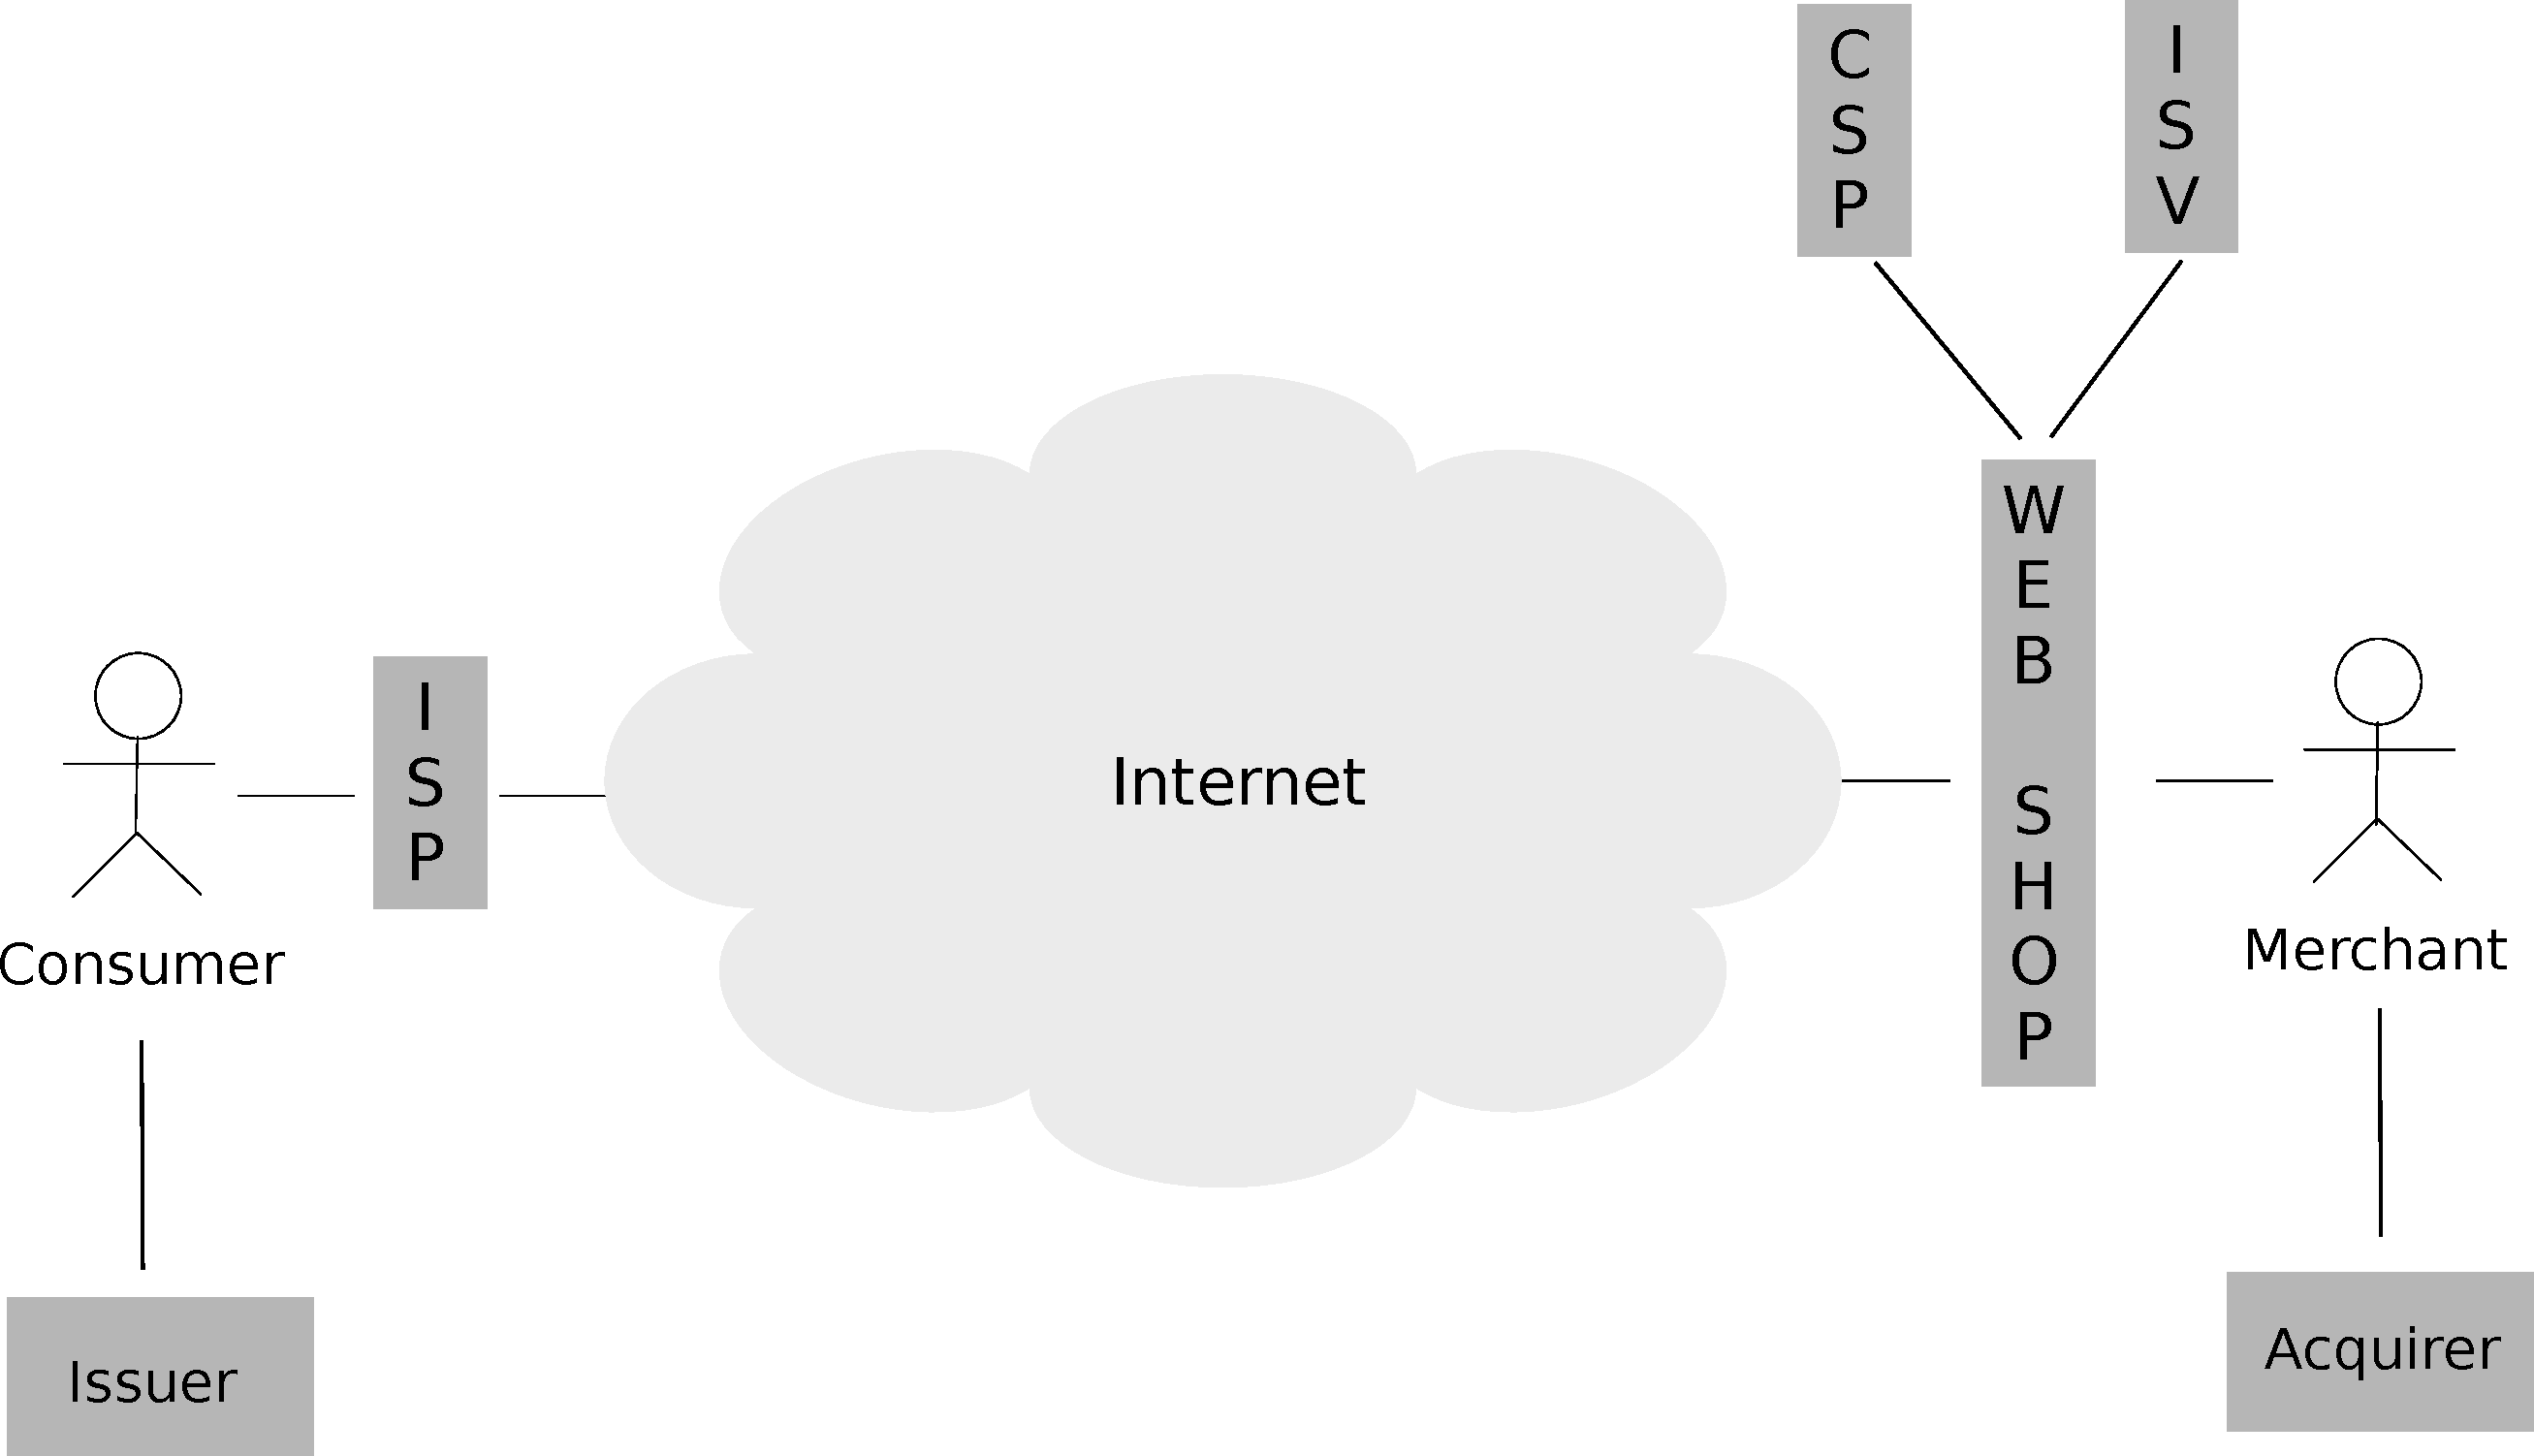
\includegraphics[width=0.8\columnwidth]{images/e-commerce-scenario.pdf}
	\caption{E-commerce Fundamentals}
\label{fig:images_ecommerce_scenario}
\end{figure}

When the consumer places the order online, the merchant receives at least a list of products or services from the current shopping cart of the consumer as well as the delivery address for the items. If the transaction is going to be finalized with a credit card, the consumer will have to state additional information like her billing address and credit card information (this includes the credit card number, the validity date and a security number). \\
The merchant does not validate the credit card information on her own. For that purpose she is usually relying on another 3$^{rd}$ party service offered on the Internet by the Payment Service Provider (PSP). These providers are either validating the credit card information themselves based on a given user profile (e.g.\ a central Web service like PayPal) or connecting to the issuing bank of the card for doing so. For this validation process the merchant is handing over the following information to the PSP:\@

\begin{itemize}
    \item consumer's billing address
    \item given credit card number, validity date and security number
    \item final amount of the transaction being processed
\end{itemize}

The PSP or the issuing bank is validating the correctness of the information: is the billing address matching the current consumers' postal address on file? Is the stated credit card information correct and is this credit card not marked as blocked? \\
The merchant will receive the status of the authorization as well as an authorization code in return. If the authorization was done successfully the merchant will collect the items and send out a shipping request to one of the available logistic services capable to handle the order. They will pickup the order at the merchant's facility and ship it to the delivery address stated by the consumer. Usually in parallel the merchant is informing her bank about the order, amount due as well as authorization code from the PSP.\@ The acquirer is in charge to withdrawal the amount of the order from the consumers bank account either via the PSP or directly with the issuing bank (a process called clearing).\@

\begin{figure}[H]
	\centering
		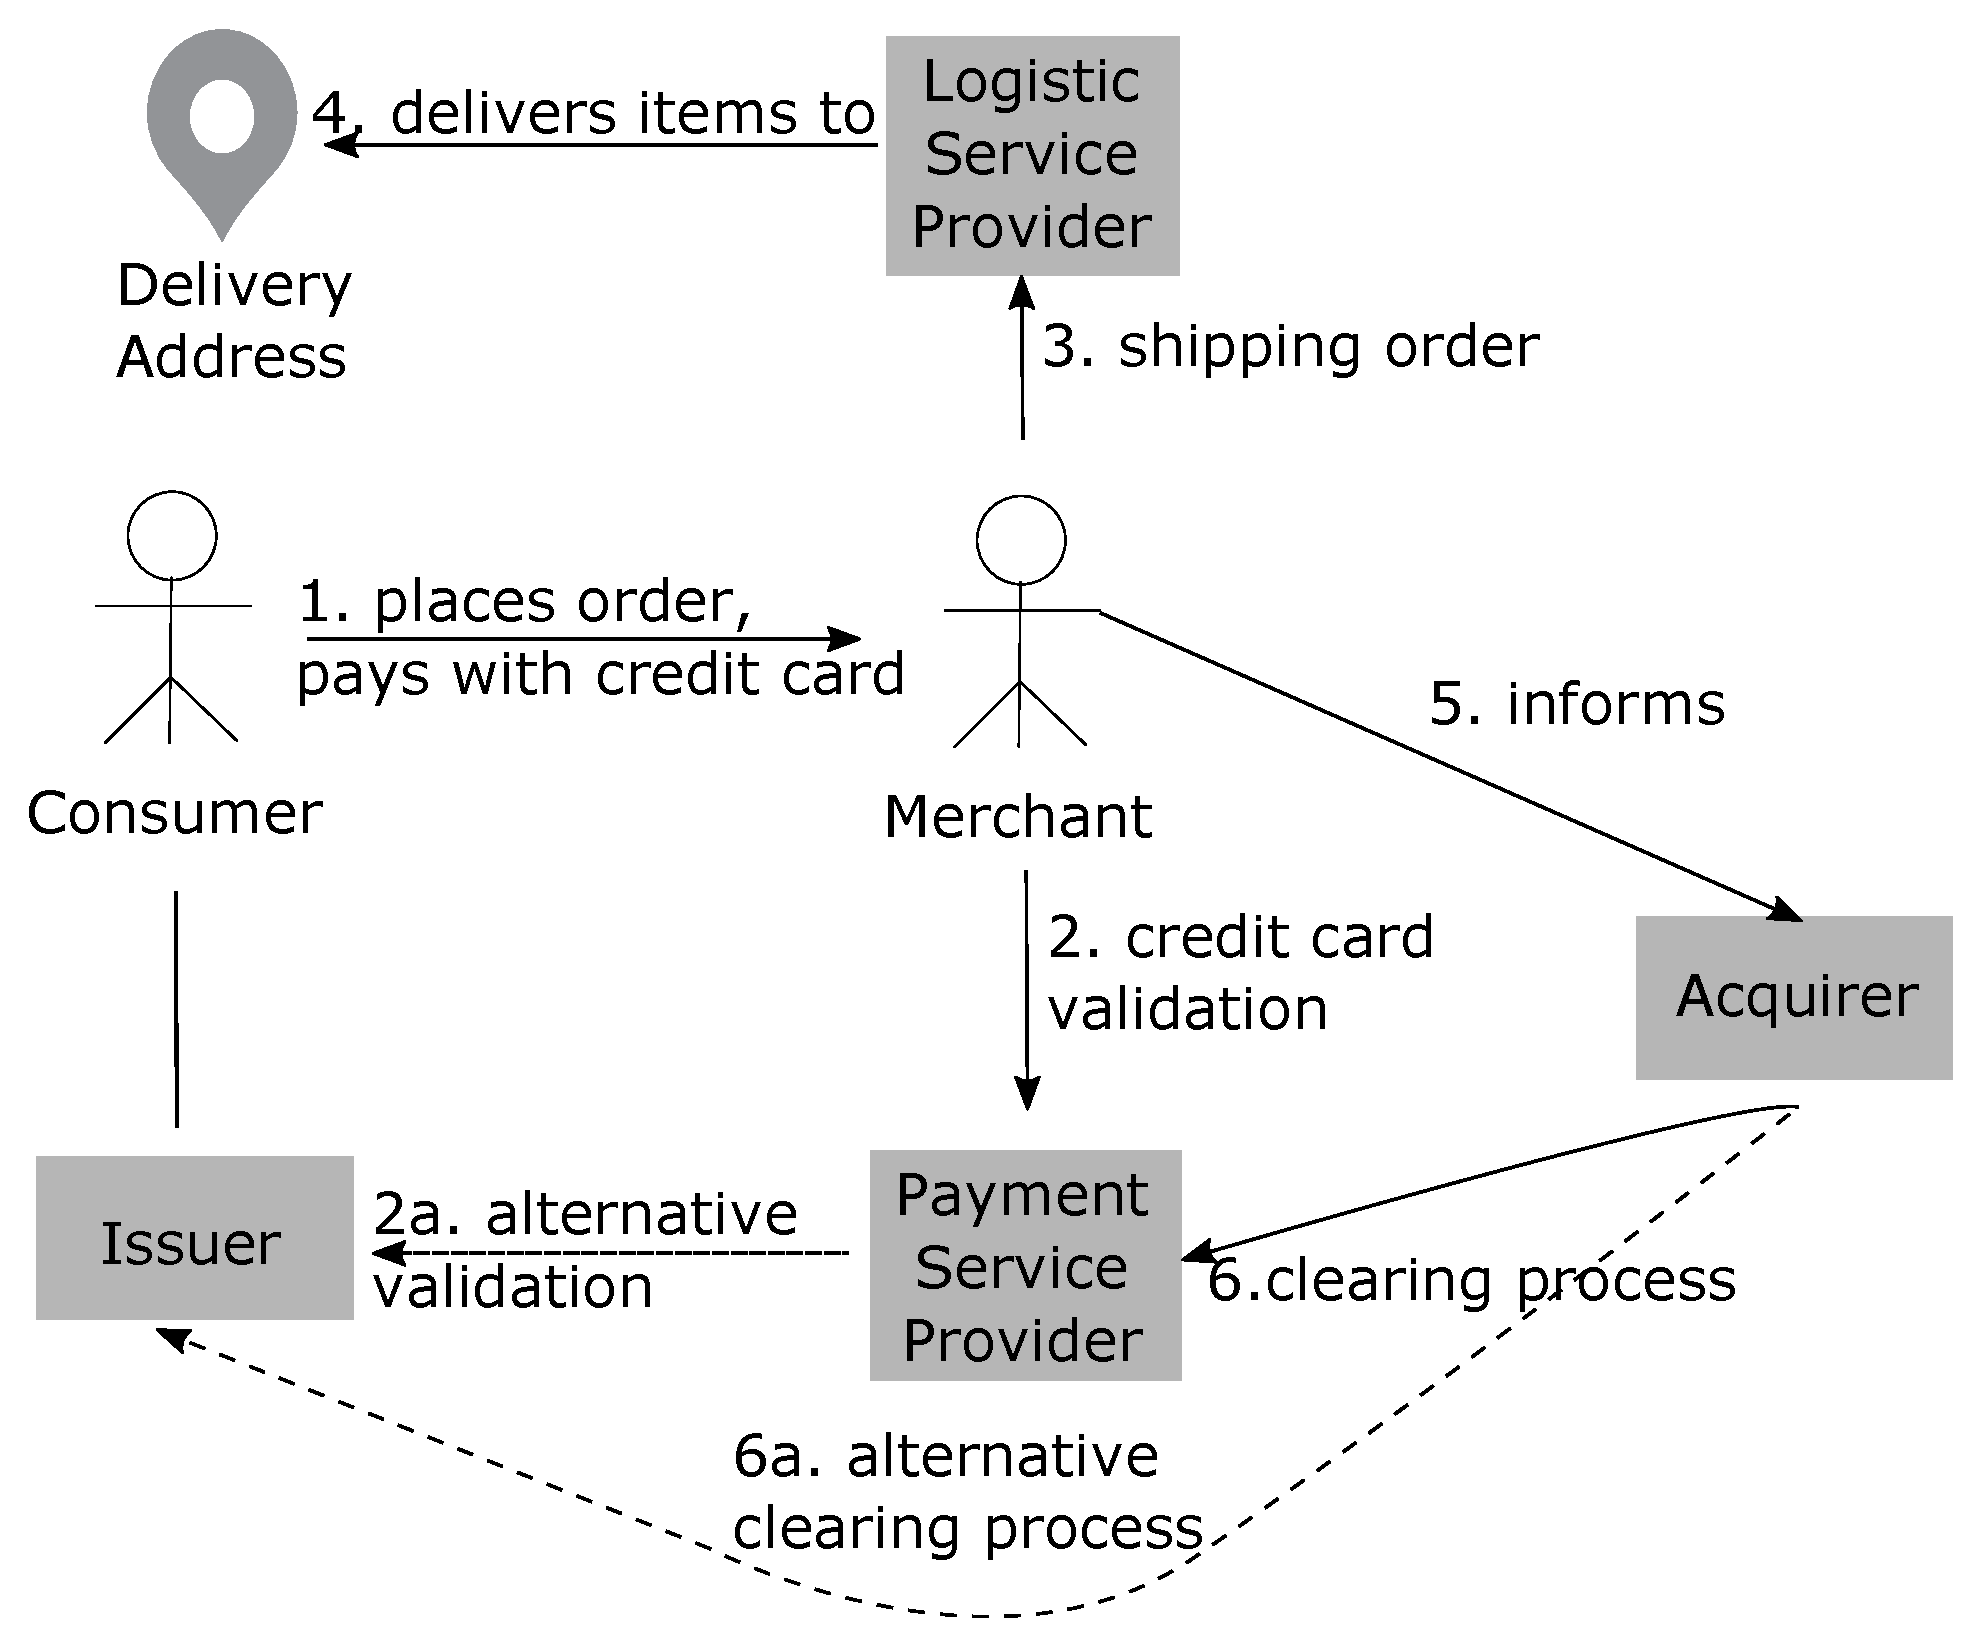
\includegraphics[width=0.8\columnwidth]{images/e-commerce-checkout-process.pdf}
	\caption{E-commerce Checkout Process in detail}
\label{fig:images_ecommerce_checkout_process}
\end{figure}

- the merchant have a business relationship with her own bank and uses the service to acquire the outstanding amounts from consumers \\
- in the clearing process the acquiring bank is settling any outstanding transaction with an issuing bank \\
\\
Workshop ErsteBank Wien: \\
- usually banks are monitoring the usage of credit / debit cards and are looking for suspicious activities \\
- this fraud prevention mechanism is working on a rule-based (non self-learning) or score-based (self-learning) software from a third party \\
- the outcome of the fraud prevention could be: yes (this is a fraudulent transaction, pls.\ block it), no (everything looks fine, pls. continue with the process) or maybe (uncertain, pls.\ let a human decide how to proceed) \\
- in case of the maybe result an alert is triggered to one of the support staff of the bank (operating 24/7/365) \\
- still this kind of fraud prevention mgmt. can not solve all issues due to the amount and frequency of the transactions, there is generally a
fraud-to-sales ratio of max. 0.11 percent in the EU (meaning 1 promille of transactions are fraudulent) \\
- still the success rate of fraud prevention is rougly 70-80 percent, means of the fraudulent transactions nearly 80 percent are blocked correctly \\
- for the rest: the consumer has to actively trigger an investigation, if the case is valid usually the issuing bank will cover the cost (in case of larger amounts an insurance will take over). \\
- the bank is responsible for pushing the consumer to file a case at police \\
- most of the filed cases could not be resolved \\
- there is no court decision yet in which circumstances the consumer might be guilty as well \\
\\
- ca. 85 percent of frauds are E-commerce frauds (EU: 70-90 percent). Hotspots are Germany, France and US. Frauds are coming from Travel-Shops or Online Merchants and the amount is on average between 500-600 EUR \\
- E-commerce frauds will usually not filed at police; in most cases the acquirer is in charge to handle the issue \\
- if it is known that a merchant has been hacked the bank is usually issuing new credit cards to all affected consumers automatically \\
- otherwise the bank has to get in contact with the acquirer and/or merchant to figure out if the transaction is fraudulent \\
- usually the banks only have credit card related information from a consumer (no detailed information about the ongoing transaction), whereas the merchant and the acquirer have the detailed records of the order at hand \\
- various regulations make it hard to shre detailed information with involved parties (even if they have special agreements signed between them) \\
- main questions for E-commerce fraud: who is the party that is the victim of the incident? Is it really a fraudulent transaction? \\
- E-commerce fraud can not be handled by technology alone, at best the fraudulent transaction can be blocked on the merchant side (due to the information given by the consumer like items, prices, delivery address, ...) \\
- in the worst case one successful fraudulent transaction in an E-commerce shop will trigger hundred and thousands of attempts -> so the awareness for the issue has to be at merchant side \\
- at the end: much effort is assumed to bring all the experts together and solve the issue by putting their individual know-how on the table \\


% section scenario description (end)
